%%%%%%%%%%%%%%%%%%%%%%%%%%%%%%%%%%%%%%%%%%%%%%%%%%%%%%%%%%%%%%%%%%% 
%                                                                 %
%                            CHAPTER Four                         %
%                                                                 %
%%%%%%%%%%%%%%%%%%%%%%%%%%%%%%%%%%%%%%%%%%%%%%%%%%%%%%%%%%%%%%%%%%% 
 
\chapter{SEQUENTIAL STREAM REASONING ARCHITECTURE}
\blfootnote{*Portions of this chapter previously appeared as: Rui Yan, Brenda Praggastis, William P. Smith, Deborah L. McGuinness. 2016 ``Towards A Cache-Enabled, Order-Aware, Ontology-Based Stream Reasoning Framework." Linked Data on the Web Workshop 2016, 25th World Wide Web Conference 2016}
Most existing stream reasoning systems employ the silent temporal assumption when ``forgetting'' the data, and are not designed to leverage the semantic importance model.
In this chapter, a sequential stream reasoning architecture (SSRA) is proposed to provide an infrastructure to deploy the semantic importance model in stream reasoning systems.

\section{Assumptions}
SSRA shares the common assumptions on ontologies and streaming data, under which existing systems work \cite{barbieri2009c} \cite{barbieri2010c} \cite{barbieri2010execution} \cite{barbieri2010incremental} \cite{anicic2011ep}.
%
\subsection{Ontology}
SSRA follows assumptions for background ontologies:
(1) the stream reasoning system leverages ontologies encoded in OWL \cite{mcguinness2004owl} to support the symbolic reasoning; 
(2) the background ontology is usable, correct, consistent, and provided by the domain experts;
(3) the background ontology is preloaded into the system before the processing starts;
(4) the background ontology doesn't change during the processing. 

A stream reasoning system doesn't necessarily have to employ ontologies to provide reasoning foundations. 
Existing systems \cite{do2011answer} \cite{gebser2012stream} leverage answer set programming (ASP) \cite{gelfond1991classical} to support reasoning.
\cite{mileo2013streamrule} encodes customized rules to enable reasoning.   
However, SSRA chooses to use ontologies for reasoning because they provide a flexible and expressive way to encode knowledge. 
Domain experts are key to composing the ontologies. 
The complexity of the ontology should be determined by the use case requirements. 
The correctness of the ontology is very crucial to determine the query results, as the knowledge for executing the query is solely provided by the background ontology. 
The domain knowledge in the ontologies usually doesn't change (frequently). 
Previous work including \cite{gao2016planning} \cite{ren2010towards} considers the change of the background knowledge.
Their method is to update the background ontology over time.
Between two adjacent updates, the background ontology remains static.
Overall, the assumptions on the background ontologies are reasonable and can be loosened with minimum efforts. 
%
\subsection{Streaming Data}
SSRA follows assumptions for the streaming data: 
(1) the streaming sources encapsulate the streaming data items as RDF stream format, and in unique named graphs;
(2) the streaming sources assign expiration timestamps to streaming data items;
(3) SSRA assigns arrival timestamps for the streaming data.

RDF streams \cite{della2009first} are RDF data annotated with timestamps that are either time-points or time-intervals.
The RDF stream format can be represented as $<\rho, \tau>$, where $\rho$ is an RDF molecule \cite{ding2005tracking}, and $\tau$ is a timestamp denoting the arrival time of $\rho$.
An RDF stream is defined as an ordered sequence of pairs \cite{barbieri2010proposal} \cite{barbieri2009c}, each of which consists of an RDF triple and a monotonically non-decreasing timestamp $\tau$, identified by a unique IRI that is a streaming source locater, and published in a named graph \cite{carroll2005named}.
The above work justifies the assumption of leveraging named graphs in the RDF streams. 

SSRA extends the RDF stream format by adding another timestamp and a unique graph ID.
Thus, an RDF stream is represented by $<\rho,\tau_{a}, \tau_{e}, G>$, where $\rho$ denotes the RDF molecule/statement, $\tau_{a}$ denotes its arrival timestamp, $\tau_{e}$ denotes its expiration timestamp and $G$ denotes its unique graph ID.

Under the silent temporal assumption, the expiration timestamps are assigned by the system via adding arrival timestamps with the logical window size \cite{barbieri2010incremental}. 
Given the information of the window and the system as a priori, the streaming source can assign expiration timestamps as exactly as what the system can do. 
Thus, the assumption on assigning expiration timestamps also cover the situation where the data itself carries the expiration timestamps, or data expires due to the new data arrival at some random time. 
%
\section{Architecture}
SSRA consists of a window and four sequential components: \textit{data consumption}, \textit{query execution}, \textit{result explanation} and \textit{data eviction}.
These four components are executed in a sequential order. 
The execution flow forms a loop to process data streams and to produce query results in a continuous fashion, as it is shown in Figure \ref{fig:4-ssra}. 

\begin{figure}[!htbp]
	\centering
	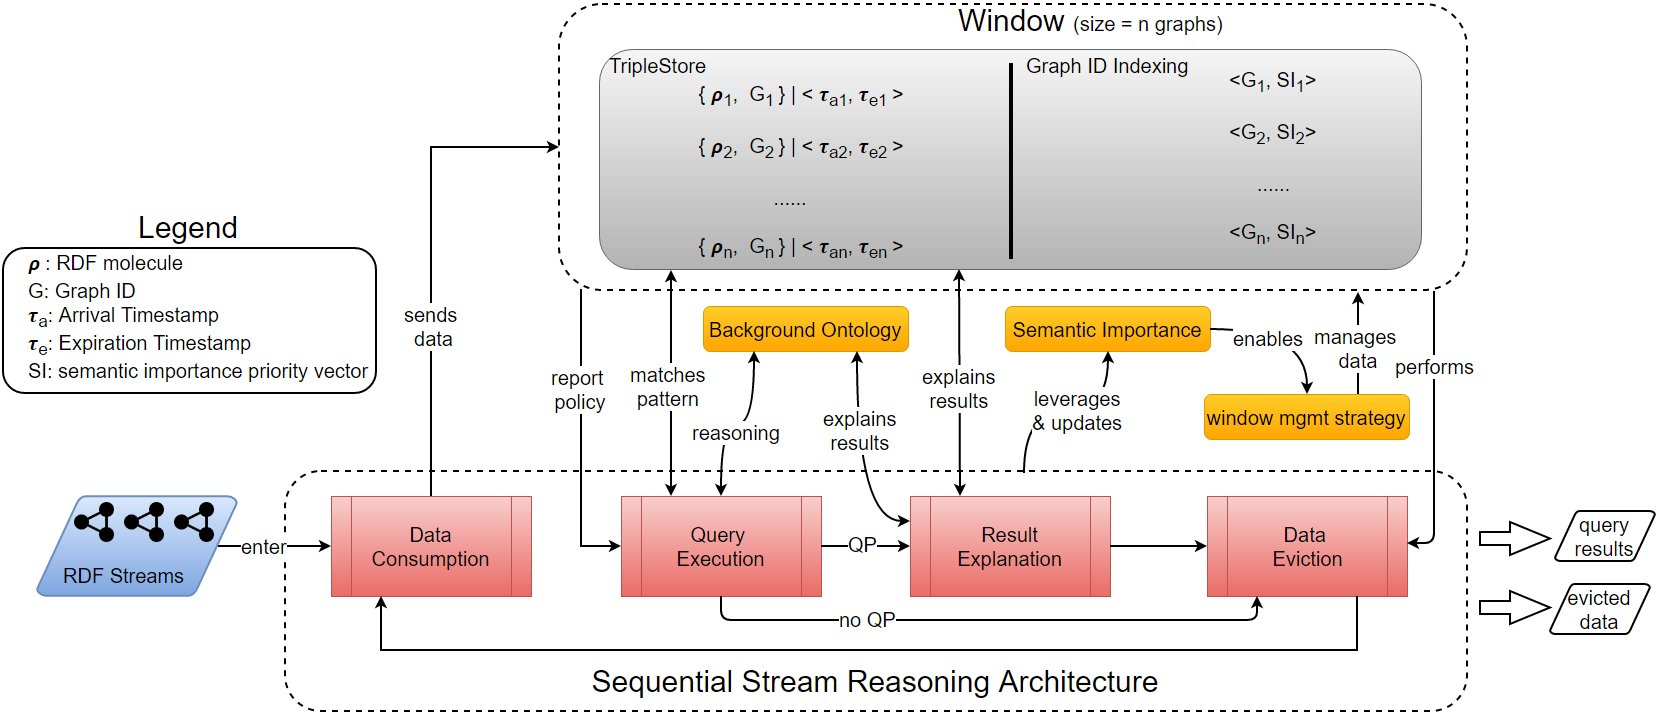
\includegraphics[angle=90,height=7.5in]{img/4-ssra.png}
	\caption{Sequential Stream Reasoning Architecture.}
	\label{fig:4-ssra}
\end{figure}

%
\subsection{Window}
The window is designed with a triple-store that stores the data physically, and a graph ID manager that indexes the data graphs.
The background ontology is preloaded in the window triple-store.
The window receives and keeps the data from the data consumption.
The query is executed in the window with the triple-store query engine, background ontology and the data.
The triple-store also provides the ability to explain the results.
The graph ID manager helps index the data, manages data semantic importance priority vectors and ranks the data. 
Coupled with the window management strategies, the graph ID manager can provide the list of data to be evicted from the triple-store.
%
\subsection{Data Consumption}
RDF streams enter SSRA via data consumption component. 
Its behavior is modeled and controlled by both Tick and Report operational semantics from the SECRET model \cite{botan2010secret}.
It consumes data in either a time-driven or tuple-driven way, depending on how the window is defined. 
It can realize different reporting policies as well. 
For example, ``on window close'' policy allows the streaming data enters the window till full before executing the query; 
while ``on content change'' policy allows to execute the query once the content is changed in the window, regardless of window fullness. 
In either policy, it will send the query execution request to the next component.
%
\subsection{Query Execution}
The query in the stream reasoning scenario should be continuous in order to provide proactive answers. 
This requires the query to be preregistered in the system before the data arrival.
SSRA, unlike what existing work does, employs standard SPARQL queries.
This is for two reasons:
(1) C-SPARQL \cite{barbieri2009c}, EP-SPARQL \cite{anicic2011ep} and other extended SPARQL queries require different execution models and syntax that are not compatible.
Even though RSP-QL \cite{dell2014rsp} was proposed later with the goal to unifying the continuous queries, it currently is meant to be a reference model to explain the heterogeneity of stream reasoning engines. 
The execution engine is very challenging to develop as it will have to cover all the C-SPARQL/CQELS/other operational semantics which possibly will lose the responsive performance.
(2) the requirement of ``continuity'' can be easily realized by forming a loop in SSRA, rather than employing some continuous query syntax or execution models. 
In fact, even the continuous SPARQL queries, such as C-SPARQL, need to be translated into the continuous query part (which includes the window and stream information), and the static query part (which is basically the SPARQL query).
Thus, the mechanism of executing a continuous SPARQL query is essentially to execute a translated SPARQL query with associated window and stream definitions.
This is the same as what SSRA does. 

In SSRA, reasoning happens during the query time. 
This provides an advantage that only the necessary entailments for the answer will be computed. 
However, it is worth pointing out that reasoning does not have to happen at the same time as the query does. 
One example is materialization \cite{barbieri2010incremental},  which is performed iteratively: the materialized snapshot of the database is always updated as long as the new data arrives. 
%
\subsection{Result Explanation}
If query participation (QP) is specified, the window needs to know the query participation status of every named graph after the query result is delivered.
Result Explanation Component works in a way to trace back to the provenance of the query result; that is to find which named graphs participated in the query process. 
The result is explained by proof trees\footnote{For an example, please refer to \url{http://docs.stardog.com/\#\_proof\_trees}}.

A(n) (inferred) result can be obtained by both explicit triples and intermediate inferences. 
Only the query participation statistics of those graph IDs belonging to explicit triples will be recorded.

In each run iteration, semantic importance has to be updated so as to re-rank the data. 
Based on different window management strategies, semantic importance is updated differently.
For example, in FEFO strategy, the window is constantly looking for expired data.
The important data is those unexpired. 
If the data expires, it will be moved to the deletion pool for eviction. 
For strategies such as FE-LFU-FO, the window updates semantic importance based on the expiration timestamp and query participation frequency.
If the data is expired, it will be moved to the deletion pool for eviction regardless how frequently it used to participate in the query. 
If the data is not expired, it will be ranked based on the frequency.
Other window management strategies will follow the same pattern to update the semantic importance.
One thing to notice is that, rules to update semantic importance is only determined by window management strategies, without human-in-the-loop required.
%
\subsection{Data Eviction}
This component evicts the named graphs ranked at the bottom in the window. 
Depending on different window management strategies, data is evicted differently.
For example, FEFO collects one statistic -- the expired data count ($E_{d}$). 
$E_{d}$ increments by one if a named graph is expired.
FE-LRU-FO collects two statistics -- $E_{d}$ and the most recent query participation timestamps ($\tau_{qp}$), for every named graph. 
$E_{d}$ increases by one if a named graph is expired.
Every valid named graph's old $\tau_{qp}$ is replaced with the corresponding new $\tau_{qp}$.
FE-LFU-FO collects two statistics -- $E_{d}$ and every named graph's query participation frequency counts ($\delta_{qp}$), in the latest cycle.
$E_{d}$ increments by one if a named graph is expired, and every valid named graph's total query participation frequency counter ($f_{qp}$), adds the corresponding $\delta_{qp}$. 
The window re-ranks the data immediately after semantic importance is updated. 
%
\section{Implementation}
In SSRA, the most important part is the window. 
All of the components are constantly interacting with the window.
SSRA implements and configures the window as follows.

\textbf{Triple-store}:
SSAR has been implemented using two off-the-shelf triple-stores: AllegroGraph v5.0.2\footnote{http://franz.com/agraph/allegrograph/} and Stardog v4.0 RC3\footnote{http://stardog.com/}. 
Both provide Java APIs and step-by-step tutorials. 
AllegroGraph is an efficient modern graph database by Franz Inc\footnote{http://franz.com/}. 
It supports up to OWL2 RL reasoning and full SPARQL 1.1. 
Stardog is a graph database by Complexible Inc\footnote{http://complexible.com/}. 
It supports up to OWL2 DL \& rule-based reasoning and SPARQL 1.1.
Stardog supports reasoning explanation via proof trees, but AllegroGraph does not. 
Free versions of both products are used.

The SPARQL drop argument is leveraged to fully remove named graphs from the window. 
We avoid using the SPARQL delete argument because it only removes the statements in the graphs, not the graph ids.
This will pollute the window's graph ID manager in Figure \ref{fig:4-ssra}.
Stardog supports both memory \& disk-based databases, while AllegroGraph only supports disk-based databases. 
We have implemented three prototypes, focusing on Stardog memory \& disk-based and AllegroGraph disk-based window stream reasoning system. 
As mentioned above, the reasoning abilities of these two triple-stores are different.
In order to perform a fair comparison, we use a query that only requires RDFS reasoning.
%

\textbf{Window Type:}
In this implementation, we employ the sliding physical window with a fixed size $l$.
This is because, according to our extended window semantics, a physical window's size is a fixed value and thus controllable. 
In our extended semantics, a physical window step is a variable that is less than the window size. 
Thus, in order to control the window step ($d$), it is set to be 25\%, 50\%, 75\% and 100\% of $l$ to see if the amount of data to be evicted has any influence on the query results.
%
\section{Evaluation}
The stream reasoning community has not yet come to consensus on the best method to evaluate stream reasoning applications. 
SRbench\cite{zhang2012srbench} was proposed as a general benchmark system designed to test streaming RDF engines. 
LSBench\cite{le2012linked} was proposed to focus on assessing different Linked Stream Data (LSD) applications' capabilities. 
CSRBench\cite{dell2013correctness} was proposed with a special emphasis on the effects of operation semantics for stream reasoning applications. 
More recently CityBench\cite{ali2015citybench} was proposed to target smart city applications. 
Other work includes Heaven \cite{tommasini2015heaven} and YABench \cite{benchmarkdemo}.

Just like Heaven benchmark, LUBM benchmark\cite{guo2005lubm} data is used in this work. 
Even though LUBM is not designed for streaming environment, data-set is carefully converted into a RDF stream format. 
LUBM provides a well-constructed ontology describing the relations among universities, professors and students etc.
It also features a data generator which accepts customized parameters to generate arbitrary ABox data.

LUBM data generator produced 6,031,109 ABox triples. 
A data source generates streaming data by disk-reading this generated data line-by-line from a static n-triples file.
The streaming data is configured  as follows:
(1) the streaming source packs either 1, 10 or 100 triples per named graph ($T_{pg}$);
(2) each graph is assigned a unique graph id and expiration timestamp by the streaming source\footnote{\url{http://streamreasoning.org/slides/2015/10/sr4ld2015-02-rsp-extensions.pdf}, Slide 7, from ``Streaming Reasoning for Linked Data 2015`` by J-P Calbimonte, D. Dell'Aglio, E. Della Valle, M. I. Ali and A. Mileo.};
(3) the system assigns an arrival timestamp to each arriving named graph in a monotonically non-decreasing order.

The streaming data is then streamed to our three prototypes, where the window is configured as follows:
(1) $l$ is either 10, 100 or 1000 graphs;
(2) $d$ is either 25\%, 50\%, 75\% and 100\% of $l$;
(3) the preregistered query, as shown in Listing 4.1, requires RDFS reasoning;
(4) the background ontology is preloaded into the system.

\begin{lstlisting}[language=SPARQL,caption=SPARQL Query,basicstyle=\small,frame=single]
PREFIX rdf:<http://www.w3.org/1888/02/22-rdf-syntax-ns#>
PREFIX lubm:<http://swat.cse.lehigh.edu/onto/univ-bench.owl#>
SELECT DISTINCT ?s
WHERE { ?s rdf:type lubm:Professor. }
\end{lstlisting}

Our evaluation platform specifications include 14.04 64bits Ubuntu LTS operating system, Intel(R) Xeon(R) CPU E5-2620 v2 @2.10GHz, 2040MB memory, and 16GB HDD. 

Together with the generated ABox data and provided LUBM ontology, a ground truth of 27,192 results are obtained, and 252 experiments are conducted.
Key performance indicators of each implementation are recorded, including memory consumption, quey runtime, result explanation and data eviction under different configuration in combination of streaming data and window. 
Result explanation time is not recorded for all the FEFO strategy and other strategies with the $d = 100\%$ of $l$, because the FEFO does not need result explanation, and it does not make sense to explain result as the whole window will be dumped. 
Using these results we ask the following questions:
\begin{enumerate}
	\item What are the effects of different windows from different producers (AllegroGraph v.s. Stardog), configurations (disk-based v.s. memory-based) and semantics (different combinations of $l$ and $s$)?
    \item How do various strategies perform under different combined configurations of the streaming data and window\footnote{Currently we are using F-measure to evaluate the performance.}?
    \item What are the trade-offs to consider when deploying SSRA in different scenarios?
\end{enumerate}

We show two figures of the total 46 visualizations\footnote{Please refer to our github repository for all visualizations: \url{https://github.com/raymondino/SequentialStreamReasoningArchitecture}} generated from the results to answer the first two questions. 
The third one will be discussed shortly. 
For the sake of convenience, the following abbreviation is used: 
prototypes are abbreviated such that SM denotes Stardog memory-based window, SD denotes Stardog disk-based window and AD denotes AllegroGraph disk-based window. 
Each test case is labeled as $<$prototype abbreviation$>$\_$<$window management strategy$>$\_$<$streaming data configuration$>$. 
For example, SD\_FE-FI-FO\_1 denotes a Stardog disk-based window with the FE-FI-FO strategy to process RDF streams with 1 triple per graph.

\begin{figure}[!htbp]
	\centering
	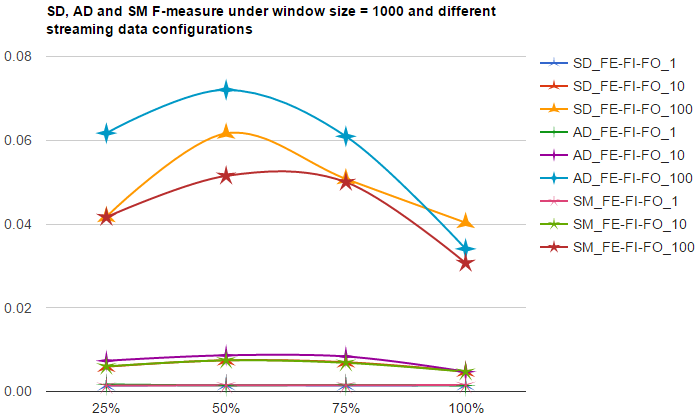
\includegraphics[width=5in]{img/4-ff.png}
	\caption{F-measure of Different Windows with FEFO}
	\label{fig:fefo}
\end{figure}

Figure \ref{fig:fefo} shows the F-measure performances brought by different windows. 
Some easy observations are: 
(1) the F-measure increases as the streaming throughput increases;
(2) the F-measure at $d = 50\%\ l$ is always best, and 100\% is always worst for all cases;
(3) AD\_FE-FI-FO performs similarly as others do when streaming throughput is 1 triple per graph, but outperforms as the streaming configuration increases;
(4) SD\_FE-FI-FO and SM\_FE-FI-FO compete with each other in each test run.

The above observations can partially answer the first question, with the points that different triple-store producers do affect the F-measure performance, but different window configurations do not have a significant influence. 
The greater the streaming input, the more influences are made on F-measure. 
However, in order to give a thorough answer we need to look at other metrics before assessing the overall performance. 
For example, AD\_FE-FI-FO gives the best F-measure, but does it take more time to execute the query and data eviction?

\begin{figure}[!htbp]
	\centering
	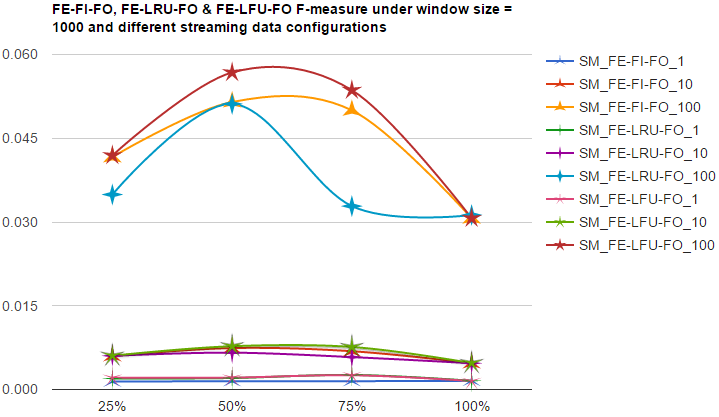
\includegraphics[width=5in]{img/4-fds.png}
	\caption{F-measure of SM Window with Different Strategies}
	\label{fig:diff}
\end{figure}

Figure \ref{fig:diff} shows the F-measure performance by different strategies for the SM windows with different streaming data configurations. 
The observations are: 
(1) F-measure increases as the streaming throughput increases;
(2) $d = 50\%\ l$ has the biggest F-measure score, 100\% has the smallest score for all the cases;
(3) for the same streaming data configuration, FE-LFU-FO always performs best, followed by FE-LRU-FO and then FE-FI-FO.

These observations can answer the second question from the perspective of big window size. 
Nevertheless, does window size affect these strategies' performances? 
Does it take longer time to explain all of the inferences? 
If yes, is it worthwhile to sacrifice system responsiveness for a better F-measure?

Additional observations are as follows:
(1) F-measure score: our raw experimental results have shown that F-measure increases as the window size increases. 
The F-measure score is also affected by different triple-stores. 
We believe this is because AlllegroGraph's and Stardog's inner implementation engines and mechanisms are different\footnote{Exploration and explanation of triple-stores' inner implementations are out of the scope of this dissertation}.    
(2) Memory consumption: when $l=10$, cases of $T_{pg}=1$ require 3 times on average the memory of bigger streaming configured cases. 
When $l=100$, the overall memory consumption decreases as the eviction amount (window step) increases. 
When $l=1000$, the overall memory consumption increases as the eviction amount (window step) increases. 
However, within this evaluation, no significant differences are observed between memory-based window and disk-based window. 
Small window and streaming throughput cases usually requires more memory.
Average FE-FI-FO strategy memory consumed is 41.93MB, FE-LRU-FO is 40.4MB and FE-LFU-FO is 39.59MB.
(3) Query time: AD requires the most query time for all cases. 
SD requires less time than AD but more than SM. 
The query time increases as window size and streaming input increases.
One potential reason for this is because a disk-based window needs some IO time when executing a query, which takes more time than a memory-based window. 
Average query time for all FE-FI-FO cases is 18ms, FE-LRU-FO is 15ms, FE-LFU-FO is 13ms.
(4) Explanation time: result explanation time increases approximately linearly as window and streaming input increases. 
In most cases, FE-LFU-FO takes longer time to explain.
Average FE-LFU-FO explanation time is 90371ms, FE-LRU-FO is 86100ms.
(5) Eviction time: eviction time increases as eviction amount, window size and streaming input increases. 
AD eviction time is very fast, 30ms on average. 
SD on average is 2879ms. 
SM on average is 4042ms.

According to the window and streaming data configurations, there can be either 10, 100, 1,000, 10,000 or 100,000 triples in the window during one processing loop. 
We identify a small case where 10 or 100 triples are processed, a medium case where 1,000 or 10,000 triples are processed, and a large case where 100,000 triples are processed. 
Together with Table \ref{tab:tradeoff}, we present a thorough comparison among triple-stores, window types and data management strategies under these scenarios, as well as to help answer the third question above-mentioned, i.e., what are the trade-offs to consider when deploying our architecture in different scenarios?

\begin{table*}[!htbp]
\centering
\caption{The Trade-off Table}
\label{tab:tradeoff}
\resizebox{\textwidth}{!}{%
\begin{tabular}{|c|c|l|r|r|r|r|r|}
\hline
Scenario & Tuple \# in window & window Config. & \multicolumn{1}{c|}{SPARQL (ms)} & \multicolumn{1}{c|}{F-measure} & \multicolumn{1}{c|}{Explain (ms)} & \multicolumn{1}{c|}{Eviction (ms)} & \multicolumn{1}{c|}{Memory (MB)} \\ \hline
\multirow{14}{*}{Small} & \multirow{7}{*}{10} &AllegroGraph& 20.25 & 4.35E-05 & - & 69.25 & 22.00 \\
&&Stardog& 5.13 & 3.93E-05 & - & 11.00 & 56.75 \\ \cline{3-8} 
&& Disk & 8.69 & 5.43E-05 & 1970.25 & 26.94 & 57.00 \\
&& Memory & 5.00 & 5.40E-05 & 1790.25 & 9.50 & 56.25 \\ \cline{3-8} 
&& FE-FI-FO & 10.17 & 4.07E-05 & 0 & 30.42 & 45.17 \\
&& FE-LRU-FO & 5.00 & 5.68E-05 & 1571.00 & 11.50 & 61.38 \\
&& FE-LFU-FO & 4.63 & 7.19E-05 & 2189.50 & 11.50 & 74.75 \\ \cline{2-8} 
& \multirow{7}{*}{100} &AllegroGraph& 11.63 & 2.97E-04 & - & 73.38 & 58.38 \\
&&Stardog& 5.00 & 3.05E-04 & - & 20.81 & 42.81 \\ \cline{3-8} 
&& Disk & 6.75 & 3.70E-04 & 8058.81 & 34.94 & 41.88 \\
&& Memory & 4.92 & 3.84E-04 & 8178.63 & 20.17 & 41.08 \\ \cline{3-8} 
&& FE-FI-FO & 5.41 & 2.27E-04 & 0 & 28.75 & 36.00 \\
&& FE-LRU-FO & 5.41 & 4.17E-04 & 7846.44 & 21.38 & 37.19 \\
&& FE-LFU-FO & 5.00 & 4.44E-04 & 8391.00 & 21.25 & 36.19 \\ \hline
\multirow{14}{*}{Medium} & \multirow{7}{*}{1,000} &AllegroGraph& 12.17 & 1.53E-03 & - & 89.42 & 59.08 \\
&&Stardog& 6.46 & 1.55E-03 & - & 164.96 & 36.21 \\ \cline{3-8} 
&& Disk & 8.35 & 1.68E-03 & 25372.54 & 129.35 & 40.52 \\
&& Memory & 6.56 & 1.74E-03 & 25265.42 & 169.14 & 36.97 \\ \cline{3-8} 
&& FE-FI-FO & 8.36 & 1.54E-03 & 0 & 139.78 & 43.53 \\
&& FE-LRU-FO & 6.96 & 1.82E-03 & 24355.21 & 151.33 & 37.54 \\
&& FE-LFU-FO & 7.04 & 1.85E-03 & 26282.75 & 151.42 & 33.21 \\ \cline{2-8} 
& \multirow{7}{*}{10,000} &AllegroGraph& 15.63 & 7.25E-03 & - & 90.00 & 33.38 \\
&&Stardog& 9.56 & 6.49E-03 & - & 1575.38 & 37.93 \\ \cline{3-8} 
&& Disk & 11.34 & 6.77E-03 & 122612.38 & 1020.72 & 39.41 \\
&& Memory & 9.22 & 6.77E-03 & 144213.08 & 1150.50 & 36.28 \\ \cline{3-8} 
&& FE-FI-FO & 11.58 & 6.75E-03 & 0 & 1080.25 & 36.42 \\
&& FE-LRU-FO & 9.50 & 6.18E-03 & 113897.38 & 1556.94 & 40.81 \\
&& FE-LFU-FO & 9.81 & 6.89E-03 & 113782.88 & 1004.19 & 32.13 \\ \hline
\multirow{7}{*}{Large} & \multirow{7}{*}{100,000} &AllegroGraph& 127.75 & 5.72E-02 & - & 187.25 & 23.50 \\
&&Stardog& 76.13 & 4.60E-02 & - & 27949.00 & 36.13 \\ \cline{3-8} 
&& Disk & 134.31 & 4.64E-02 & 261564.75 & 17122.81 & 31.13 \\
&& Memory & 15.17 & 4.22E-02 & 271454.38 & 32248.08 & 36.67 \\ \cline{3-8} 
&& FE-FI-FO & 93.33 & 4.97E-02 & 0 & 18695.08 & 31.92 \\
&& FE-LRU-FO & 84.88 & 3.57E-02 & 263054.63 & 27104.50 & 33.63 \\
&& FE-LFU-FO & 66.50 & 4.58E-02 & 269964.50 & 27470.63 & 35.75 \\ \hline
\end{tabular}
}
\end{table*}
Each value in the table is calculated from raw experimental results.
Please refer to our github repository for these raw results. 
In the 10 triples/window scenario, for example, 
disk-based window's F-measure score is averaged from AD\_FE-FI-FO, SD\_FE-FI-FO, SD\_FE-LRU-FO \& SD\_FE-LFU-FO test cases, 
while memory-based window's score is averaged from SM\_FE-FI-FO, SM\_FE-LRU-FO \& SM\_FE-LFU-FO test cases.
We would like to highlight an empirical comparison of the two window types, the disk-based window (DC) and the memory-based window (MC).

The detailed comparisons of all aspects for different scenarios are provided as follows:
(1) SPARQL query time: for every scenario, DC is slower than MC. 
As the scenario increases, DC grows much faster than MC. 
The ratio between 100,000 triples/window and 10 triples/window for DC is 15.45, whilst MC is 3.34. 
Though DC is less restricted by storage space, its query time slows down the system response time, and this effect will become worse as the scenario size grows.
However, this is expected, as accessing disk when executing query is always slower than accessing the memory.     
(2) F-measure: for every scenario, DC's and MC's F-measure scores are very similar. 
This means both types are able to provide same level correctness.
F-measure increases as scenario increases, this is because the more data in the window, the more correct results can be calculated, which raises the F-measure.	
(3) Reasoning Explanation Time: in most scenarios, MC's explanation time is slower than DC's. 
The difference increases significantly as the scenario size increases.
Reasoning explanation is very time-consuming. 
Strategies (such as FE-LFU-FO) requiring reasoning-explanation provide better F-measure when the scenario is small and explanation time is quick, but provide similar F-measure when the scenario is large and explanation time is slow.	
(4) Eviction Time: in small scenarios, DC is slower; in medium and large scenarios, MC is slower.
The difference between DC and MC increases significantly as the scenario size increases. 
This indicates a bias towards DC for large RDF streams, and MC for small RDF streams.	
(5) Memory Consumption: Both DC and MC consume similar memory for each scenario. 
This could be because Stardog triple-stores are implemented very efficiently, but again, explaining this requires the knowledge of inner mechanisms of Stardog, which is out of the scope of this work. 

Under the small case, AllegroGraph's query and eviction time is several times that of Stardog. 
Disk and memory performs equally on F-measure, though disk requires more time to query, evict and explain. 
FE-LFU-FO performs best in F-measure, followed by FE-LRU-FO then FEFO. 
Though FEFO needs more time to query and evict, the explanation time required by FE-LRU-FO and FE-LFU-FO is significantly greater. 
The trade-offs in deploying our framework under the small scenario is dependent on the use case. 
If system responsiveness is the first class citizen, a FEFO strategy will be chosen since it does not require explanation and provides a fine F-measure. 
Stardog memory window can be chosen since it provides faster execution time and better F-measure. 
If F-measure is most important, FE-LFU-FO is the right strategy.
Stardog memory window is the best as memory window provides less explanation time. 
It is also noticed that $d = $ 25\% or 50\% of $l$ provides better F-measure.

For medium cases, Stardog's eviction time increases significantly.
Though Stardog's query time is better than AllegroGraph's, the difference is very small when compared with the eviction time.
Disk window provides less eviction time; its other metrics are similar as memory windows.
FE-LFU-FO is the best at F-measure scores, but is traded for longer explanation time.
Actually FEFO provides decent F-measure without explanation time.
Overall, AllegroGraph disk window with FEFO is most suitable for this scenario.
$d=50\%$ or $75\%$ of $l$ provides best F-measure as well.

For large cases, AllegroGraph's eviction time, F-measure and memory performs better, though query is slower.
Disk window query time is 9 times greater than the memory dependent graph database, but provides better F-measure, explanation , eviction time and memory. 
FEFO performs best in F-measure but it spends more time on query, with smallest eviction time and memory consumption. 
Hence, AllegroGraph disk window with FEFO is most suitable for this experiment's use case. It is also recommended to use $d = 50\% $ of $l$ to provide the best F-measure.
%
\section{Summary}
This chapter introduces the sequential stream reasoning architecture, and shows how semantic importance model can be used in stream reasoning applications. 
The window is implemented with two off-the-shelf triple-stores (Stardog or AllegroGraph), with different configurations (memory-based or disk-based).
The benchmark leverages LUBM dataset by streaming it, and constantly looking for the answers of the query ``who is a professor?'', which requires RDFS reasoning.
This can be seen to look for professors on a time line by streaming the LUBM dataset. 
In order to illustrate how to use semantic importance in stream reasoning with SSRA, four aspects $\tau_{a}$, $\tau_{e}$, $f_{qp}$ and $\tau_{qp}$ are chosen to form three window management strategies:
FE-FI-FO with its priority vector $[\tau_{a}, \tau_{e}]$, FE-LFU-FO with $[\tau_{e}, f_{qp}, \tau_{a}]$, and FE-LRU-FO with $[\tau_{e}, \tau_{qp}, \tau_{a}]$. 
The SSRA implementations have demonstrate a physical sliding window, but the temporal window is easy to implement as well according to the extended window semantics.
The architecture operational semantics is very flexible, as the data consumption component is able to realize different operational semantics. 
In all three implementations, the report policy is ``on window close''.
The continuous processing is enabled by the inner loop of the architecture. 
The query is a pure SPARQL query, which is different from most of the existing work. 
The window is implemented in the triple-store, with a graph ID manager that indexes graph IDs, and updates data semantic importance priority vectors.
The benchmark results show that the architecture is scalable, but for strategies involved with query participation aspects, as the window size increases, the result explanation time increases significantly.
Thus, in order to use query participation aspect, the window size has either to be kept relatively small, which is one of the incentives that semantic importance is proposed, 
or to use some filtering functionality such as query relevance aspect in the semantic importance model in order to reduce the data in the window. 
In the next chapter, we will show how to keep the window size small with the architecture and semantic importance, as well as show how the proposed model and infrastructure can be leveraged for real-life use cases.